\chapter{Implementierung}

\section{Implementierung des Servers}
\subsection{Parsen der Informationen mit Jsoup}
Um die nötigen Informationen über Foren, Threads und Beiträge für die App
bereitzustellen, müssen diese aus dem bestehenden HTML von readmore.de
ausgelesen werden. Dazu wird das im vorherigen Kapitel schon beschriebene
Framework \Fachbegriff{jsoup} eingesetzt. Um die Informationen auszulesen,
wurden für Foren, Threads und Beiträge jeweils ein eigener Parser implementiert
wie im nachfolgenden UML-Diagramm zu sehen ist.
\begin{figure*}[!htbp]
\centering
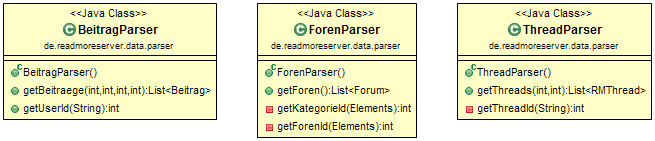
\includegraphics[width=\textwidth]{Bilder/Parser.png}
\caption[Parser für die verschiedenen Forenbereiche]{Parser für die verschiedenen Forenbereiche
 \protect\footnote{eigene Darstellung.} }
\label{dminfo}
\end{figure*}
Jeder der Parser liefert eine Liste vom Typ des jeweiligen geparsten Objekts
zurück, also entweder \Code{Forum}, \Code{RMThread} oder \Code{Beitrag}. Diese
Objekte werden zur internen Datenhaltung verwendet und wärend des Parsens des
HTML erstellt und mit Daten befüllt. Zusätzlich zu Foren, Threads und Beiträgen,
werden auch die Benutzer in einem eigenen Objekt abgebildet. Dort werden
notwendige Informationen zur späteren Darstellung in der App abgebildet, wie z.B
der Benutzername und der Link zum Avatar des Benutzers. Das Enum \Code{RMStatus}
bildet die Sichtbarkeit des Online Status eines Benutzers ab. Im nachfolgenden
UML-Diagramm wird der Aufbau der einzelnen Objekte dargestellt.
\begin{figure*}[!htbp]
\centering
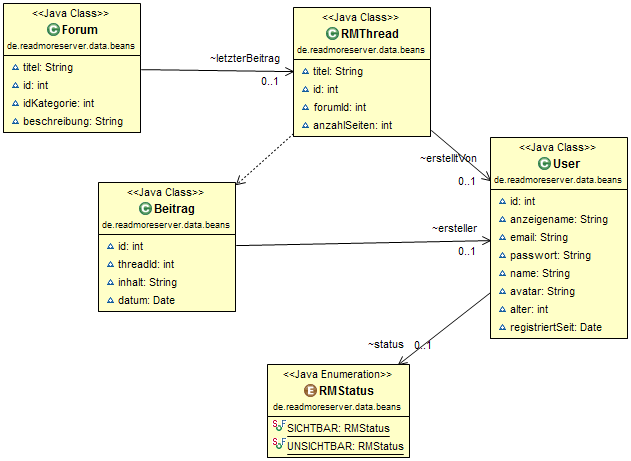
\includegraphics[width=\textwidth]{Bilder/beans.png}
\caption[Objekte für die interne Datenhaltung]{Objekte für die interne Datenhaltung \protect\footnote{eigene Darstellung.} }
\label{dminfo}
\end{figure*}
\subsection{REST Schnittstelle}

\section{Implementierung der App}